\section{Blockchain suffix proofs}

We now provide a concrete non-interactive PoPoW construction which allows
proving certain predicates $Q$ of the chain $\chain$. The construction will
be done in two steps: First, we will build a construction which is limited to
a class of predicates that is easy to prove. Later, we will extend this class
of predicates by augmenting the construction.

Among the predicates which are stable, we now limit ourselves to the class of
predicates which are functions of only the chain suffix $\chain[-k - 1:]$. We
call these predicates $(k+1)$-\textit{suffix sensitive}. As we will illustrate,
these predicates are significantly easier to prove, but at the same time allow
us to use the construction as a scaffold for the more generic case.

\begin{definition}[Suffix sensitivity]
A chain predicate $Q$ is called $k$-\textnormal{suffix sensitive} if for all
chains $\chain, \chain'$ with $|\chain| \geq k$ and $|\chain'| \geq k$ such that
$\chain[-k:] = \chain'[-k:]$ we have that $Q(\chain) = Q(\chain')$.
\end{definition}

Given this suffix-sensitivity definition, we deduce that for each
suffix-sensitive predicate $Q$ there must exist a ``short version'' predicate
$\tilde{Q}$ which can deduce the value of $Q(\chain)$ by only examining the
suffix of the chain, that is $Q(\chain) = \tilde{Q}(\chain[-k:])$.

Suffix-sensitive predicates allow proving that a recent transaction occurred in
the longest chain and in a block buried under at most $k$ blocks. Because
the predicates we are interested in are stable, they must also pertain to
properties that are independent of the last $k$ blocks. Therefore, combining the
two, the predicate can only describe something that is visible at the exact
block $\chain[-k-1]$ and that will also remain true as the chain grows in
perpetuity (due to monotonicity). These predicates may seem contrived for
blockchains like Bitcoin. However, they make sense for blockchains such as
Ethereum which maintain state \cite{vitalik} that is propagated and committed to
in every block. The existence of a stable monotonic state bit flip, for example
the creation of an indestructible smart contract, can therefore be described
using such predicates.

\subsection{Construction}

We will now describe the details of the NIPoPoW construction by presenting a
specific prover and verifier. We present a generic form of the verifier first
and the prover afterwards. The generic form of the verifier will work with any
practical suffix proof protocol (we make this more exact below). Therefore, it
makes sense to describe the generic verifier first before we talk about the
specific instantiation of our protocol. The generic verifier is given access to
call a proof comparison operator $\leq_m$ which is protocol-specific. We
therefore begin the description of our protocol by first illustrating the
generic verifier. Next, we describe the prover specific to our protocol.
Finally, we show the instantiation of the $\leq_m$ operator, which plugs into
the generic verifier to make a concrete verifier for our protocol.

\subsubsection{The generic verifier}

The \textsf{Verify} function of our NIPoPoW construction is described in
Algorithm~\ref{alg.nipopow-verifier}. The verifier algorithm is parameterized by
a chain predicate $Q$ and security parameters $k$ and $m$. The parameter $k$
pertains to the amount of proof-of-work needed to bury a block so that it is
believed to remain stable; in bitcoin's case, we often set $k = 6$. The
parameter $m$ is a security parameter pertaining to the prefix of the proof,
which connects the Genesis block to the $k$-sized suffix.  The verifier receives
several proofs by different provers in a collection of proofs $\mathcal{P}$, at
least one of which must be generated by an honest prover. Iterating over these
proofs, it extracts the best one by comparing these proofs.

Each of these proofs is a chain. For honest provers, these
chains are subchains of the currently adopted chain. The proofs consist of two
parts, $\pi$ and $\chi$, such that $\pi \chi$ is a valid chain. $\chi$ is called
the proof suffix, for which we require that $|\chi| = k$, while $\pi$ is called
the proof prefix. For honest provers, $\chi$ will be the last $k$ blocks of
their adopted chain, while $\pi$ will consist of a selected subset of blocks
from the rest of their chain preceding $\chi$. The exact method of choice of
this subset will become clear when we describe the concrete prover in the next
section.

The verifier compares the various proofs provided to it by calling the $\geq_m$
comparison operator, which is defined by the protocol. We will get to the
operator's definition after we have examined the prover algorithm. All proofs
are checked for validity before comparison by checking that $|\chi| = k$ and
subsequently using the \textit{validChain} function. This function simply checks
that $\pi\chi$ is an anchored blockchain by ensuring that the first block in the
proof is the common reference string (Genesis) and that each block in the proof
contains a pointer to the previous block within the proof.

\import{./}{algorithms/alg.verifier-lite.tex}

At each loop iteration, the verifier compares the next candidate proof prefix
$\pi$ against the currently best known proof prefix $\tilde\pi$ by calling $\pi
\geq_m \tilde\pi$. If the candidate prefix is better than the currently best
known proof prefix, then the currently known best prefix is updated by setting
$\tilde\pi \leftarrow \pi$. When the best known prefix is updated, the suffix
$\tilde\chi$ associated with the best known prefix is also updated to match the
suffix $\chi$ of the candidate proof by setting $\tilde\chi \leftarrow \chi$.
While $\tilde\chi$ is needed for the final predicate evaluation, it is not used
as part of any comparison, as it has the same size $k$ for all proofs. The best
known proof prefix is initially set to $(Gen)$, the trivial anchored chain
containing only the genesis block. Any well-formed proof compares favourably
against the trivial chain.

After the end of the for loop, the verifier will have determined the best proof
$(\tilde\pi, \tilde\chi)$. We will later prove that this proof will necessarily
belong to an honest prover with overwhelming probability. Since the proof has
been generated by an honest prover, it is associated with an underlying honestly
adopted chain $\chain$. The verifier then evaluates the predicate $Q$ on the
underlying chain associated with the proof by invoking $\tilde{Q}$.

This generic form of the verifier will work for any protocol for suffix proofs,
as long as the underlying operator $\leq_m$ is defined in a manner that is
transitive and returns the same result if invoked multiple times with the same
inputs with overwhelming probability.

\subsubsection{The concrete prover}

The NIPoPoW honest prover construction is shown in
Algorithm~\ref{alg.nipopow-prover}. The honest prover is supplied with an
honestly adopted chain $\chain$ and security parameters $m, k, \delta$ and
returns a proof $\pi\chi$, which is a chain. The proof consists of a suffix
$\chi$ and a prefix $\pi$. The suffix $\chi$ is simply the last $k$ blocks of
$\chain$. The prefix $\pi$ is constructed by selecting various blocks and adding
them to $\pi$. which consists of a number of blocks for every level $\mu$. At
the highest possible level at which at least $m$ blocks, all these blocks are
presented. Then, inductively, for every superchain of level $\mu$ that is
included in the proof, the suffix of length $m$ is taken. Then the underlying
superchain of level $\mu - 1$ covering the same span as that suffix is also
included, until level $0$ is reached. This underlying superchain will have $2m$
blocks in expectation and always at least $m$ blocks.

\import{./}{algorithms/alg.nipopow-prover.tex}

The algorithm returns a chain $\pi\chi$. In this chain, $\chi$ is the suffix of
the blockchain containing the most recent $k$ blocks. $\pi$ is a subchain of the
underlying blockchain with the last $k$ blocks removed, $\chain[:-k]$. In each
iteration of the for loop, blocks of level $\mu$ are considered, starting from
the top-most level $|\chain[-k].\textsf{interlink}|$ and descending down to
level $0$.

When we take a
$\mu$-superchain and are interested in its last $m$ blocks, we fill the same
range of blocks with blocks from the superchain of level $\mu - 1$ below. All
the blocks of level $\mu$ which are within this last $m$ blocks range will also
be superblocks of level $\mu - 1$ and so we do not want to keep them in the
proof structure twice.  Note furthermore that no check is necessary to make sure
the top-most level has at least $m$ blocks, even though the verifier requires
this. The reason is the following: Assume the blockchain has at least $m$ blocks
in total. Then when a superchain of level $\mu$ has less than $m$ blocks in
total, these blocks will all be necessarily included into the proof by a
lower-level superchain $\mu - i$ for some $i > 0$. Therefore, it does not hurt
to add them to the set $\pi$ earlier.

Figure~\ref{fig.nipopow} contains an example proof constructed for parameters
$m = k = 3$. The top superchain level which contains at least $m$ blocks is
level $\mu = 3$. For the $m$-sized suffix of that level, $5$ blocks of
superblock level $2$ are included for support spanning the same range. For the
last $3$ blocks of the level $2$ superchain, blocks of level $1$ are included
for support.

\begin{figure}[h]
    \caption{
    Non-interactive proof-of-work prefix $\pi$ for $m = 3$ on a chain good
    everywhere.
    }
    \centering
    \iftwocolumn
        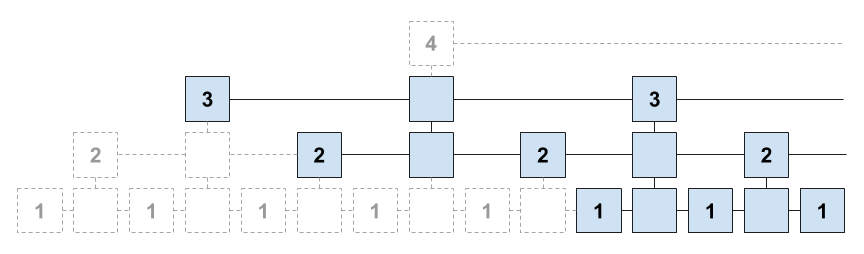
\includegraphics[width=\columnwidth,keepaspectratio]{figures/non-interactive-popow.png}
    \else
        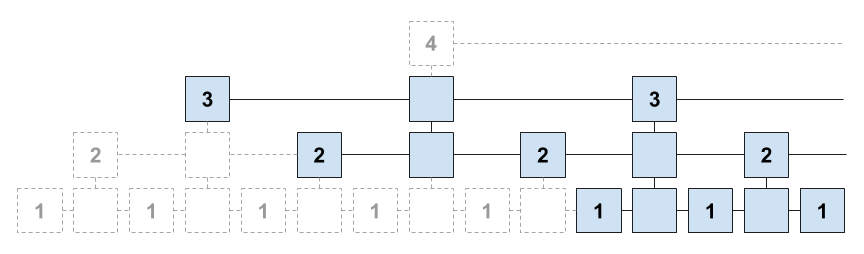
\includegraphics[width=0.7\columnwidth,keepaspectratio]{figures/non-interactive-popow.png}
    \fi
    \label{fig.nipopow}
\end{figure}

\subsubsection{The concrete verifier}

Finally, the $\geq_m$ operator which performs the actual comparison of proofs
is presented in Algorithm~\ref{alg.nipopow-maxchain}. It takes two proofs as
parameters and returns true if the first proof is winning, otherwise it return
false to indicate the second proof is winning. Initially the algorithm parses
the sets of blocks into chains by arranging them in topological order. It
rejects proofs that are not valid chains. It then computes the lowest common
ancestor block $b$ between the two proofs by calling the LCA function. Finally,
it finds the highest superblock level in which at least one of the proofs has
at least $m$ blocks. If the other one doesn't, then the one who does wins.
Otherwise, the one with most blocks wins. The number of blocks is counted using
the findInChain function, which returns the index of a block within the
respective superchain.

\import{./}{algorithms/alg.nipopow-maxchain.tex}
